%%%%%%%%%%%%%%%%%%%%%%%%%%%%%%%%%%%%%%%%%%%
%
% From a template maintained at https://github.com/jamesrobertlloyd/cbl-tikz-poster
%
%%%%%%%%%%%%%%%%%%%%%%%%%%%%%%%%%%%%%%%%%%%

\documentclass[portrait,a0b,final,a4resizeable]{a0poster}
\setlength{\paperwidth}{36in} % A0 width: 46.8in
\setlength{\paperheight}{48in} % A0 width: 46.8in

\usepackage{atbegshi}% http://ctan.org/pkg/atbegshi
\AtBeginDocument{\AtBeginShipoutNext{\AtBeginShipoutDiscard}}
\usepackage{qrcode}
\usepackage{multicol}
\usepackage{enumitem}
\usepackage{mathtools}
%\usepackage{color}
%\usepackage{morefloats}
%\usepackage[pdftex]{graphicx}
%\usepackage{rotating}
\usepackage{amsmath, amsthm, amssymb, bm}
%\usepackage{array}
%\usepackage{booktabs}
\usepackage{multirow}
%\usepackage{hyperref}
\usepackage{pgf-soroban}
\usepackage{bussproofs}
\usetikzlibrary{cd,shapes.geometric,arrows,chains,matrix,positioning,scopes,calc}
\tikzstyle{mybox} = [draw=white, rectangle]
%\definecolor{darkblue}{rgb}{0,0.08,0.45}
%\definecolor{blue}{rgb}{0,0,1}
%\usepackage{dsfont}
\usepackage[margin=0.5in]{geometry}
%\usepackage{fp}

%%%%%%%%%%%%%%%%%%%%%%%%%%%%%%%%%%%%%%%%%%%
%
% myfig
%
% \myfig - replacement for \figure
% necessary, since in multicol-environment
% \figure won't work
%
%%%%%%%%%%%%%%%%%%%%%%%%%%%%%%%%%%%%%%%%%%%

\newcommand{\myfig}[3][0]{
    \begin{center}
        \vspace{1.5cm}
        \includegraphics[width=#3\hsize,angle=#1]{#2}
        \nobreak\medskip
    \end{center}}

%%%%%%%%%%%%%%%%%%%%%%%%%%%%%%%%%%%%%%%%%%%
%
% mycaption
%
% \mycaption - replacement for \caption
% necessary, since in multicol-environment \figure and
% therefore \caption won't work
%
%%%%%%%%%%%%%%%%%%%%%%%%%%%%%%%%%%%%%%%%%%%

%\newcounter{figure}
\setcounter{figure}{1}
\newcommand{\mycaption}[1]{
    \vspace{0.5cm}
    \begin{quote}
    {{\sc Figure} \arabic{figure}: #1}
    \end{quote}
    \vspace{1cm}
    \stepcounter{figure}
}

%%%%%%%%%%%%%%%%%%%%%%%%%%%%%%%%%%%%%%%%%%%
%
% Some standard colours
%
%%%%%%%%%%%%%%%%%%%%%%%%%%%%%%%%%%%%%%%%%%%

\definecolor{camlightblue}{rgb}{0.601 , 0.8, 1}
\definecolor{camdarkblue}{rgb}{0, 0.203, 0.402}
\definecolor{camred}{rgb}{1, 0.203, 0}
\definecolor{camyellow}{rgb}{1, 0.8, 0}
\definecolor{lightblue}{rgb}{0, 0, 0.80}
\definecolor{white}{rgb}{1, 1, 1}
\definecolor{whiteblue}{rgb}{0.80, 0.80, 1}

%%%%%%%%%%%%%%%%%%%%%%%%%%%%%%%%%%%%%%%%%%%
%
% Some look and feel definitions
%
%%%%%%%%%%%%%%%%%%%%%%%%%%%%%%%%%%%%%%%%%%%

\setlength{\columnsep}{0.03\textwidth}
\setlength{\columnseprule}{0.0018\textwidth}
\setlength{\parindent}{0.0cm}

%%%%%%%%%%%%%%%%%%%%%%%%%%%%%%%%%%%%%%%%%%%
%
% \mysection - replacement for \section*
%
% Puts a pretty box around some text
% TODO - any other thoughts for what this box should look like
%
%%%%%%%%%%%%%%%%%%%%%%%%%%%%%%%%%%%%%%%%%%%

\tikzstyle{mysection} = [rectangle,
draw=none,
shade,
outer color=camlightblue!30,
inner color=camlightblue!30,
text width=0.965\columnwidth,
text centered,
rounded corners=20pt,
minimum height=0.09\columnwidth]

\newcommand{\mysection}[1]
{
    \begin{center}
        \begin{tikzpicture}
            \node[mysection] {\sffamily\bfseries\LARGE#1};
        \end{tikzpicture}
    \end{center}
}

%%%%%%%%%%%%%%%%%%%%%%%%%%%%%%%%%%%%%%%%%%%
%
% Set the font
%
% TODO - Not sure what a canonical choice is - feel free to modify
%
%%%%%%%%%%%%%%%%%%%%%%%%%%%%%%%%%%%%%%%%%%%

\renewcommand{\familydefault}{cmss}
\sffamily

%%%%%%%%%%%%%%%%%%%%%%%%%%%%%%%%%%%%%%%%%%%%%%%%%%%%
%%%               Background                     %%%
%%%%%%%%%%%%%%%%%%%%%%%%%%%%%%%%%%%%%%%%%%%%%%%%%%%%

\newcommand{\background}[3]{
%\definecolor{cgradbegin}{#1}
%\definecolor{cgradend}{#2}
% \psframe[fillstyle=gradient,gradend=cgradend,
% gradbegin=cgradbegin,gradmidpoint=#3](0.,0.)(1.\textwidth,-1.\textheight)
}




%%%%%%%%%%%%%%%%%%%%%%%%%%%%%%%%%%%%%%%%%%%%%%%%%%%%
%%%                pcolumn                       %%%
%%%%%%%%%%%%%%%%%%%%%%%%%%%%%%%%%%%%%%%%%%%%%%%%%%%%

\newenvironment{pcolumn}[1]{
    \begin{minipage}{#1\textwidth}
        \begin{center}
        }{
        \end{center}
    \end{minipage}
}



%%%%%%%%%%%%%%%%%%%%%%%%%%%%%%%%%%%%%%%%%%%%%%%%%%%%
%%%                pbox                          %%%
%%%%%%%%%%%%%%%%%%%%%%%%%%%%%%%%%%%%%%%%%%%%%%%%%%%%

\definecolor{lcolor}{rgb}{0, 0, 0.80}
\definecolor{gcolor1}{rgb}{1, 1, 1}
\definecolor{gcolor2}{rgb}{.80, .80, 1}

% \def\fc{fillcolor}
% \def\getfc #1=#2\par{\def\ffc{#1} \ifx\ffc\fc #2\fi}
% \def\getfillcolor #1,#2\par{\getfc #1\par \getfc #2\par}

%  \newcommand{\psshadowbox}[2]{%[2][magenta]{
%      \fbox{Input arg: #1}
%      \fbox{#1}
%      \fbox {\getfillcolor #1\par}
%      \def\col{\getfillcolor #1\par}

%      \let\coll=\col
%       \coll
%     \colorbox{\col}{#2}
%       \mbox
%   \coloredshadowbox{black}{\coll}{#2}
%   }

\newcommand{\pbox}[4]{
%\psshadowbox[#3]{
%\fbox{
    \mbox{
        \begin{minipage}[t][#2][t]{#1}
            #4
        \end{minipage}
    }%}
}

%%%%%%%%%%%%%%%%%%%%%%%%%%%%%%%%%%%%%%%%%%%
%
% Poster environment
%
% Centres everything and can be used to define the width of the content
%
%%%%%%%%%%%%%%%%%%%%%%%%%%%%%%%%%%%%%%%%%%%

\newenvironment{poster}{
    \begin{center}
        \begin{minipage}[c]{\textwidth}
        }{
        \end{minipage}
    \end{center}
}

\def\newarrow{\mbox{\begin{tikzpicture}
                        \useasboundingbox{(-3pt,-4.5pt) rectangle (19pt,1pt)};
                        \draw[->] (0,-0.07)--(17pt,-0.07);\end{tikzpicture}}}

%%%%%%%%%%%%%%%%%%%%%%%%%%%%%%%%%%%%%%%%%%%
%
% Bottom box
%
%%%%%%%%%%%%%%%%%%%%%%%%%%%%%%%%%%%%%%%%%%%

\newlength{\bottomboxheight}
\setlength{\bottomboxheight}{0.1\paperheight}

\newcommand{\bottombox}[1]{\vfill
\noindent\colorbox{white}{
    \begin{minipage}[c][\bottomboxheight][c]{\textwidth}
        \centering
        \begin{minipage}{0.9\textwidth}
            \vfill{

                \fontsizesection\color{black}
                #1
            }

        \end{minipage}
    \end{minipage}

}
}

%% Bottom box logo
\newcommand{\bottomboxlogo}[2][width=\textwidth]{
    \begin{minipage}[c][\bottomboxheight][c]{0.3\textwidth}
        \raggedleft\includegraphics[#1]{#2}
    \end{minipage}
}

\newcommand{\bottomboxlogoleft}[2][width=\textwidth]{
    \begin{minipage}[l][\bottomboxheight][c]{0.3\textwidth}
        \raggedleft\includegraphics[#1]{#2}
    \end{minipage}
}

%%%%%%%%%%%%%%%%%%%%%%%%%%%%%%%%%%%%%%%%%%%
%
% Highlighting
%
%%%%%%%%%%%%%%%%%%%%%%%%%%%%%%%%%%%%%%%%%%%

\definecolor{slightgray}{rgb}{0.90, 0.90, 0.90}

\usepackage{soul}
\makeatletter
\def\SOUL@hlpreamble{%
    \setul{}{3.0ex}%
    \let\SOUL@stcolor\SOUL@hlcolor%
    \SOUL@stpreamble%
}
\makeatother

\newcommand{\inline}[1]{%
    \begingroup%
    \sethlcolor{slightgray}%
    \hl{\ttfamily\small #1}%
    \endgroup
}

\newcommand{\tinline}[1]{%
    \begingroup%
    \sethlcolor{slightgray}%
    \hl{\ttfamily #1}%
    \endgroup
}

%%%%%%%%%%%%%%%%%%%%%%%%%%%%%%%%%%%%%%%%%%%
%
% Kotlin syntax highlighting
%
%%%%%%%%%%%%%%%%%%%%%%%%%%%%%%%%%%%%%%%%%%%

\usepackage[skins,breakable,listings]{tcolorbox}

\usepackage[dvipsnames]{xcolor}
\usepackage[table]{xcolor}
\lstdefinelanguage{kotlin}{
    comment=[l]{//},
    commentstyle={\color{gray}\ttfamily},
    emph={delegate, filter, firstOrNull, forEach, it, lazy, mapNotNull, println, @Repeat, return@},
    emphstyle={\color{OrangeRed}},
    identifierstyle=\color{black},
    keywords={abstract, actual, as, as?, break, by, class, companion, continue, data, do, dynamic, else, enum, expect, false, final, for, fun, get, if, import, in, infix, interface, internal, is, null, object, open, operator, override, package, private, public, return, sealed, set, super, suspend, this, throw, true, try, typealias, val, var, vararg, when, where, while, tailrec, reified},
    keywordstyle={\color{blue}\bfseries},
    morecomment=[s]{/*}{*/},
    morestring=[b]",
    morestring=[s]{"""*}{*"""},
    ndkeywords={@Deprecated, @JvmField, @JvmName, @JvmOverloads, @JvmStatic, @JvmSynthetic, Array, Byte, Double, Float, Int, Integer, Iterable, Long, Runnable, Short, String},
    ndkeywordstyle={\color{BurntOrange}\bfseries},
    sensitive=true,
    stringstyle={\color{ForestGreen}\ttfamily},
    literate={`}{{\char0}}1
}

%%%%%%%%%%%%%%%%%%%%%%%%%%%%%%%%%%%%%%%%%%%
%
% Color boxes
%
%%%%%%%%%%%%%%%%%%%%%%%%%%%%%%%%%%%%%%%%%%%

\tcbset{
    enhanced jigsaw,
    breakable,
    listing only,
    boxsep=-1pt,
    top=-1pt,
    bottom=-0.5pt,
    right=-0.5pt,
    overlay first={
        \node[black!50] (S) at (frame.south) {\Large\ding{34}};
        \draw[dashed,black!50] (frame.south west) -- (S) -- (frame.south east);
    },
    overlay middle={
        \node[black!50] (S) at (frame.south) {\Large\ding{34}};
        \draw[dashed,black!50] (frame.south west) -- (S) -- (frame.south east);
        \node[black!50] (S) at (frame.north) {\Large\ding{34}};
        \draw[dashed,black!50] (frame.north west) -- (S) -- (frame.north east);
    },
    overlay last={
        \node[black!50] (S) at (frame.north) {\Large\ding{34}};
        \draw[dashed,black!50] (frame.north west) -- (S) -- (frame.north east);
    },
    before={\par\vspace{10pt}},
    after={\par\vspace{\parskip}\noindent}
}

\newtcblisting{kotlinlisting}[1][]{%
    width=39cm,
    left=20pt,
    top=5pt,
    listing options={
        language=kotlin,
        basicstyle=\ttfamily\normalsize,
%numberstyle=\footnotesize,
        showstringspaces=false,
        tabsize=2,
        breaklines=true,
        numbers=none,
        inputencoding=utf8,
        escapeinside={(*}{*)},
        #1
    },
    underlay unbroken and first={%
        \path[draw=none] (interior.north west) rectangle node[white]{\includegraphics[width=10mm]{../figures/kotlin_file.png}} ([xshift=-18mm,yshift=-20mm]interior.north west);
    }
}

\newtcblisting{pythonlisting}[1][]{
    width=17cm,
    left=20pt,
    top=5pt,
    listing options={
        language=Python,
        basicstyle=\ttfamily\normalsize,
        upquote=true,
        breaklines=true,
        showstringspaces=false,
        keywordstyle=\color{blue}\bfseries,
        escapeinside={(*}{*)},
        #1
    },
    fonttitle=\ttfamily\small,
    underlay unbroken and first={
        \path[draw=none] (interior.north west) rectangle node[white]{\includegraphics[width=10mm]{../figures/python_icon.png}} ([xshift=-18mm,yshift=-20mm]interior.north west);
    }
}

% Imitate syntax error
\usepackage{ulem}
\makeatletter
\def\uwave{\bgroup \markoverwith{\lower7.5\p@\hbox{\sixly \textcolor{red}{\char58}}}\ULon}
\font\sixly=lasy6 % does not re-load if already loaded, so no memory problem.
\makeatother

\usepackage{tikz}
\usepackage[skins,breakable,listings]{tcolorbox}
\usepackage{pgfplots}
\usepackage{tikz-qtree}
\usepackage{graphicx}


\usepackage{include/preamble}


% Custom notation
\newcommand{\fdeep}{\vf^{(1:L)}}
\newcommand{\flast}{\vf^{(L)}}
\newcommand{\Jx}{J_{\vx \rightarrow \vy}}
\newcommand{\Jxx}{J_{\vx \rightarrow \vy}(\vx)}
\newcommand{\Jy}{J_{\vy \rightarrow \vx}}
\newcommand{\Jyy}{J_{\vy \rightarrow \vx}(\vy)}
\newcommand{\detJyy}{ \left| J_{\vy \rightarrow \vx}(\vy) \right|}

\newcommand\transpose{{\textrm{\tiny{\sf{T}}}}}
\newcommand{\note}[1]{}
\newcommand{\hlinespace}{~\vspace*{-0.15cm}~\\\hline\\\vspace*{0.15cm}}
\newcommand{\embeddingletter}{g}
\newcommand{\bo}{{\sc bo}}
\newcommand{\agp}{Arc \gp}

\newcommand{\D}{\mathcal{D}}
\newcommand{\X}{\mathbf{X}}
\newcommand{\y}{y}
\newcommand{\data} {\X, \y}
\newcommand{\x}{\mathbf{x}}
\newcommand{\f}{\mathit{f}}

\newcommand{\fx}{ f(\mathbf{x}) }
\newcommand{\U}{\mathcal{U}}
\newcommand{\E}{\mathbf{E}}


\newcommand{\bardist}[0]{\hspace{-0.2cm}}

\newlength{\arrowsize}
\pgfarrowsdeclare{biggertip}{biggertip}{
    \setlength{\arrowsize}{10pt}
    \addtolength{\arrowsize}{2\pgflinewidth}
    \pgfarrowsrightextend{0}
    \pgfarrowsleftextend{-5\arrowsize}
}{
    \setlength{\arrowsize}{1pt}
    \addtolength{\arrowsize}{\pgflinewidth}
    \pgfpathmoveto{\pgfpoint{-5\arrowsize}{4\arrowsize}}
    \pgfpathlineto{\pgfpointorigin}
    \pgfpathlineto{\pgfpoint{-5\arrowsize}{-4\arrowsize}}
    \pgfusepathqstroke
}


% Custom commmands.

\def\jointspacing{\vspace{0.3in}}

\def\boxwidth{0.21\columnwidth}
\newcommand{\gpdrawbox}[1]{
    \setlength\fboxsep{0pt}
    \hspace{-0.36in}
    \fbox{\hspace{-4mm}
%\includegraphics[width=\boxwidth]{../figures/deep_draws/deep_gp_sample_layer_#1}
    \hspace{-4mm}}}

\newcommand{\mappic}[1]{
%\hspace{-0.05in}\includegraphics[width=\boxwidth]{../../figures/seed-0-map/latent_coord_map_layer_#1}
}

\newcommand{\mappiccon}[1]{
%\hspace{-0.05in}\includegraphics[width=\boxwidth]{../../figures/seed-0-map-connected/latent_coord_map_layer_#1}
}

\newcommand{\spectrumpic}[1]{
%\includegraphics[trim=4.5mm 0mm 4mm 3mm, clip, width=0.44\columnwidth]{../figures/spectrum/layer-#1}
}

\newcommand{\feat}{\vh}





\begin{document}
\begin{poster}
    \vspace{1\baselineskip}   % Add some space at the top of the poster


    %%% Header
    \begin{center}
        \begin{pcolumn}{1.03}
            %%% Title
            \begin{minipage}[c][9cm][c]{0.85\textwidth}
                \begin{center}
                {\veryHuge \textbf{Idiolect: A Reconfigurable Voice Coding Assistant}}\\[10mm]
                {\huge Breandan Considine, Nicholas Albion, Xujie Si\\[7.5mm]
                }
                \end{center}
            \end{minipage}
        \end{pcolumn}
    \end{center}

    \vspace*{1.5cm}

    \large


    %%%%%%%%%%%%%%%%%%%%%%%%%%%%%%%%%%%%%%%%%%%%%%%%%%%%%%%%%%%%%%%%%%%%%%
    %%% Beginning of Document
    %%%%%%%%%%%%%%%%%%%%%%%%%%%%%%%%%%%%%%%%%%%%%%%%%%%%%%%%%%%%%%%%%%%%%%

    \Large

    \begin{multicols}{2}


        \begin{aquote}{--Charles Sanders Peirce, How to Make Our Ideas Clear (1878)}
            To ascertain the meaning of an intellectual conception one should consider what practical consequences might result from the truth of that conception—and the sum of these consequences constitute the entire meaning of the conception.
        \end{aquote}

        \vspace{20pt}

        \begin{aquote}{--Ludwig Wittgenstein, Philosophical Investigations
        (1953)}
            The language is meant to serve for communication between a builder A and an assistant B. A is building with building-stones: there are blocks, pillars, slabs and beams. B has to pass the stones, in the order in which A needs them. For this purpose they use a language consisting of the words `block', `pillar', `slab', `beam'. A calls them out; — B brings the stone which he has learnt to bring at such-and-such a call. Conceive this as a complete primitive language.
        \end{aquote}
        \vspace{10pt}

        \mysection{Main Idea}
        \null\hspace*{3cm}\begin{minipage}[c]{0.85\columnwidth}
        \begin{itemize}[labelsep=1em]
            \setlength\itemsep{0.5em}
            \item Verbally instruct a computer to program itself as a human being does.
            \item How do humans interact with computers? Using a screen and a keyboard.
            \item Visually parse the workspace and offer affordances as navigable choices.
        \end{itemize}
        \end{minipage}

        \jointspacing

        \mysection{AceJump}

        \null\hspace*{1.8cm}\begin{minipage}[c]{0.90\columnwidth}
            Helps developers search and navigate source code by assigning tags to search results in an unambiguous way while minimizing total keystrokes.\\
            \href{https://github.com/acejump/acejump}{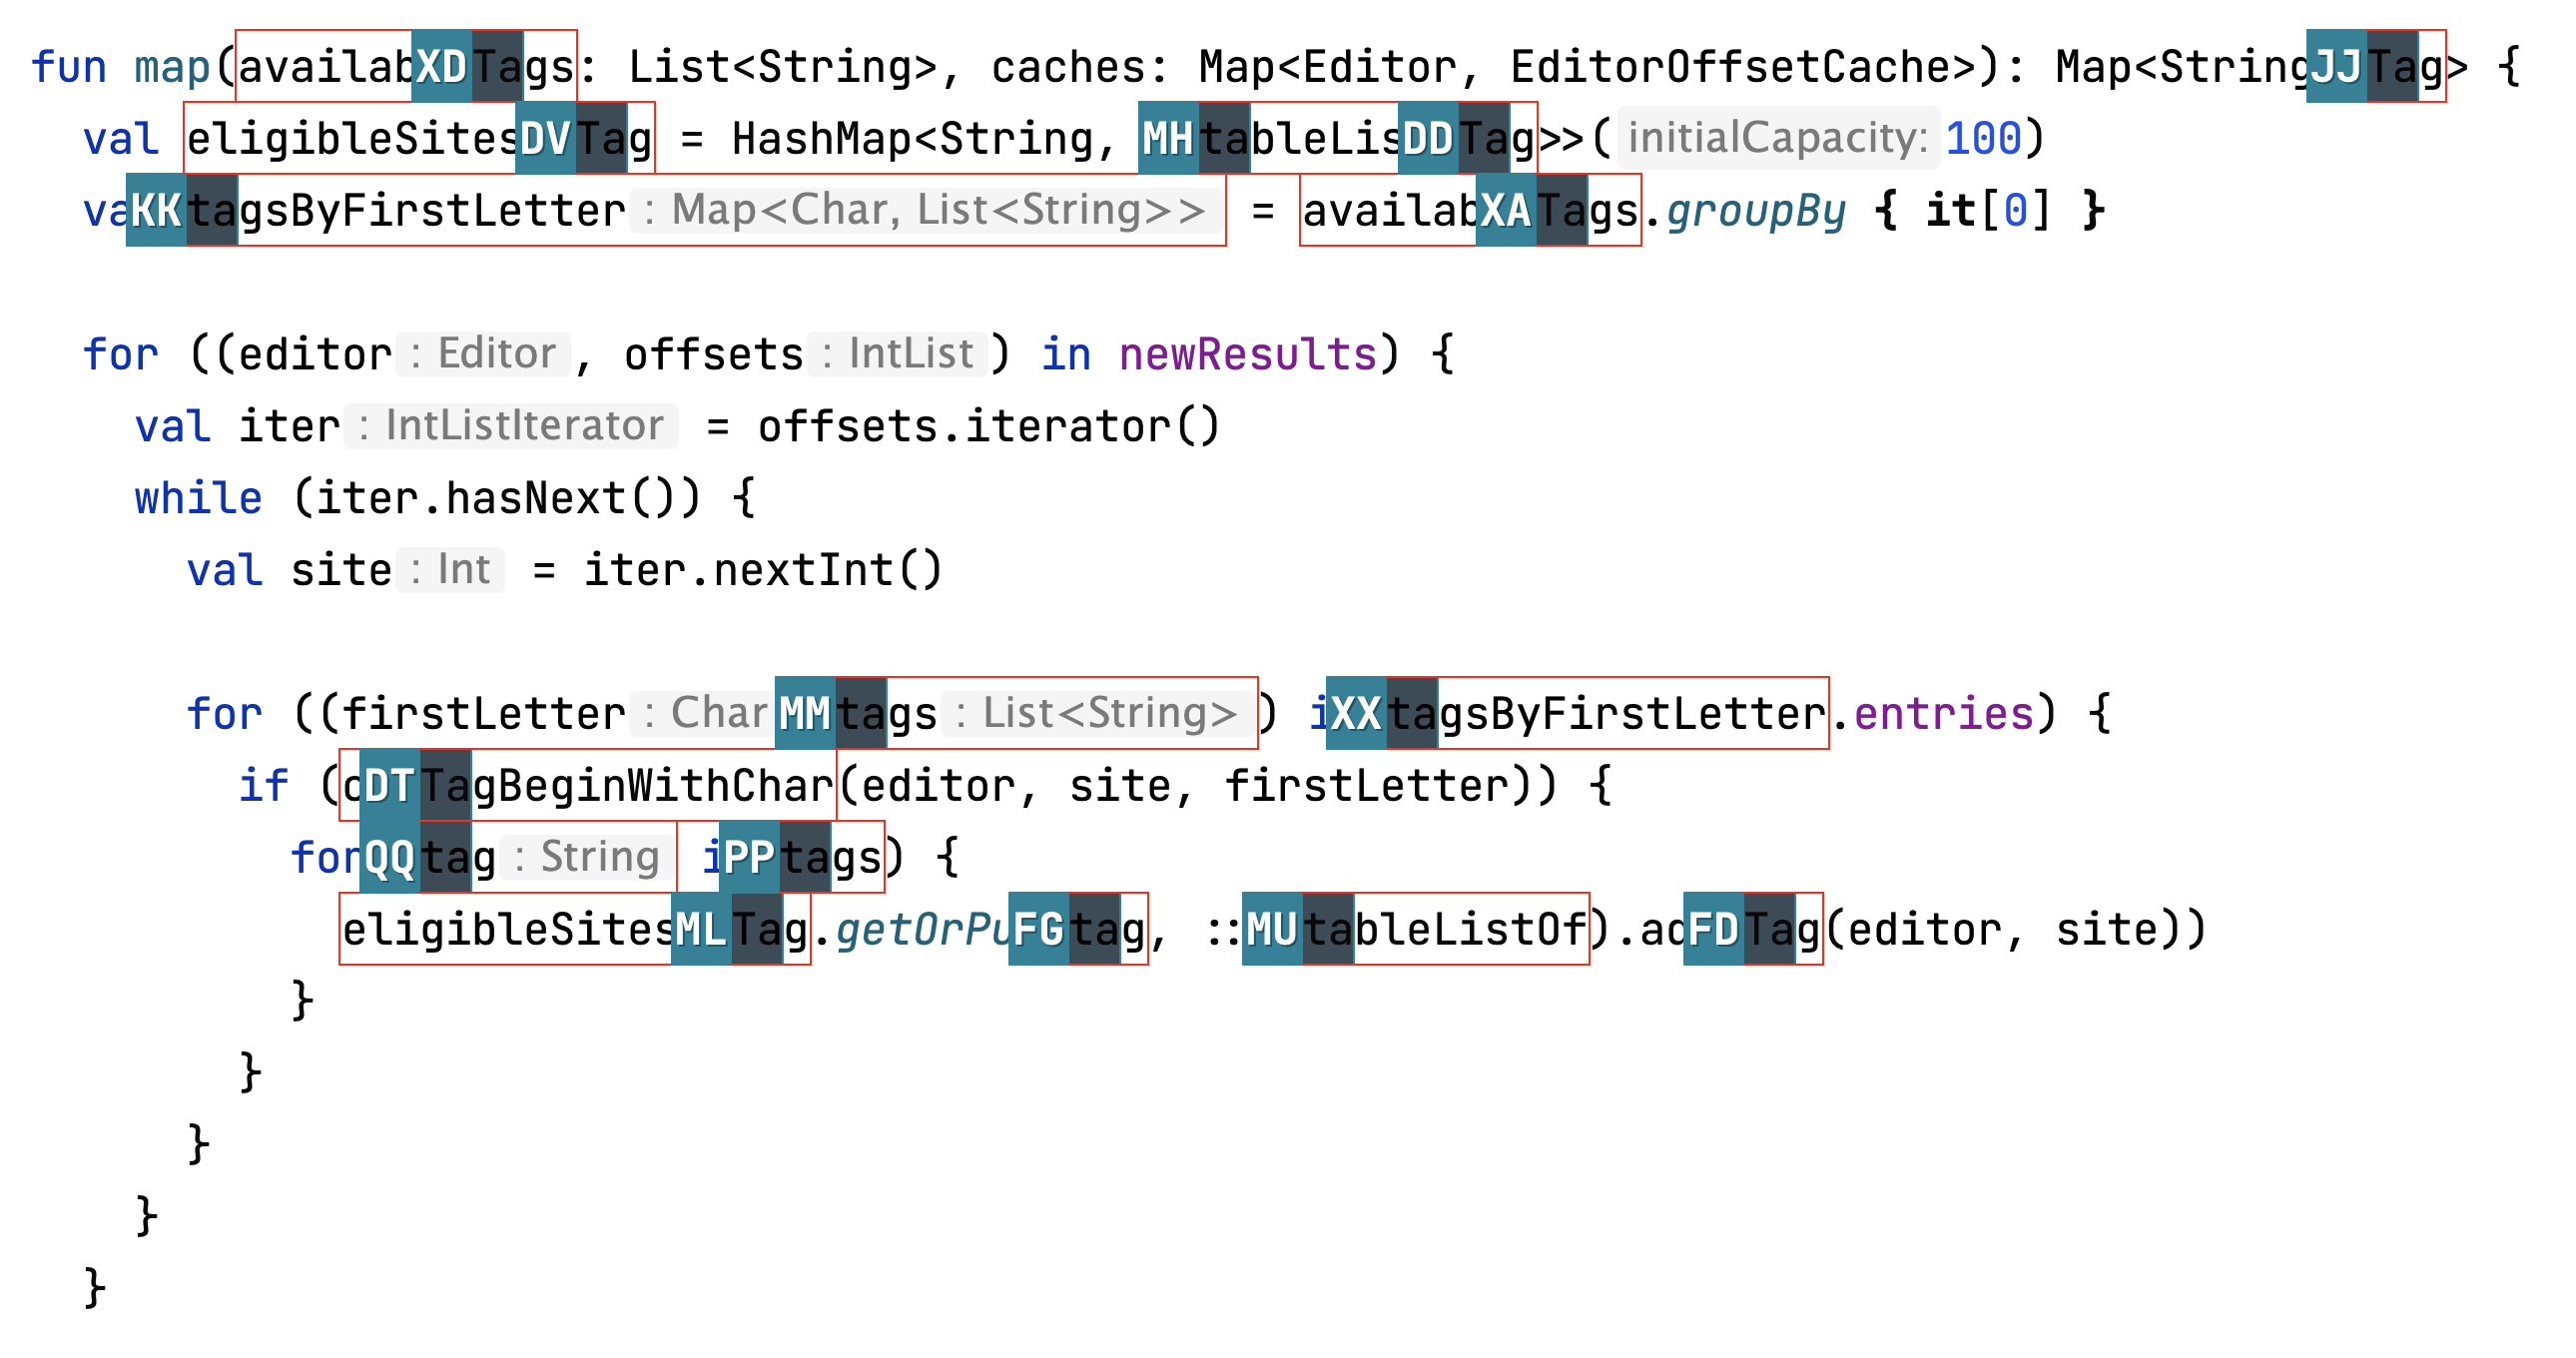
\includegraphics[width=\textwidth]{acejump_screenshot.png}}


        Given a set of indices $I$ in document $d$, and a set of tags $T$, find a bijection $f: T^*\subset T \leftrightarrow I^*\subset I$, maximizing $|I^*|$, such that:

        \begin{equation*}
            d[i\ldots k] + t \notin d[i'\ldots(k + |t|)], \forall i' \in I\setminus\{i\}, \forall k \in (i, |d| - |t|]
        \end{equation*}

        where $t \in T, i \in I$. This can be relaxed to $t=t[0]$ and $\forall k \in (i, i+K]$ for some fixed $K$, in most natural documents.

        \vspace{10pt}
        \textbf{Natural language:}
        \textit{Maximizes tags assigned to search results in uniquely-selectable manner, i.e., should never be possible to select a tag by mistake.}
        \end{minipage}

        \jointspacing

        \mysection{TraceJump}
        \null\hspace*{1.8cm}\begin{minipage}[c]{0.90\columnwidth}
                              Screenreading, object detection and visual navigation from raw screen pixels. \\

                              \hspace{-10pt}\begin{tabular}{ c c c }
                                  \includegraphics[width=12.94cm]{tracejump1.png} &
                                  \includegraphics[width=12.94cm]{tracejump2.png} &
                                  \includegraphics[width=12.94cm]{tracejump3.png}\\
                                  \small{\textbf{Activate}} & \small{\textbf{Select}} & \small{\textbf{Jump}}
                              \end{tabular}
        \end{minipage}
        \jointspacing

        \mysection{SourceJump}

        \null\hspace*{1.8cm}\begin{minipage}[c]{0.90\columnwidth}
                                Learn to retrieve contextually relevant source code from an unindexed corpus by learning to write a query which captures semantically similar documents.\\

                                \href{https://github.com/acejump/sourcejump}{\includegraphics[width=\textwidth]{sourcejump.png}}\\
        \end{minipage}

        \jointspacing

        \mysection{Tidyparse}

        \null\hspace*{1.8cm}\begin{minipage}[c]{0.90\columnwidth}
                                Suggests minimal syntax repairs ranked by naturalness and Levenshtein distance.\\

                                \href{https://github.com/tidyparse/tidyparse}{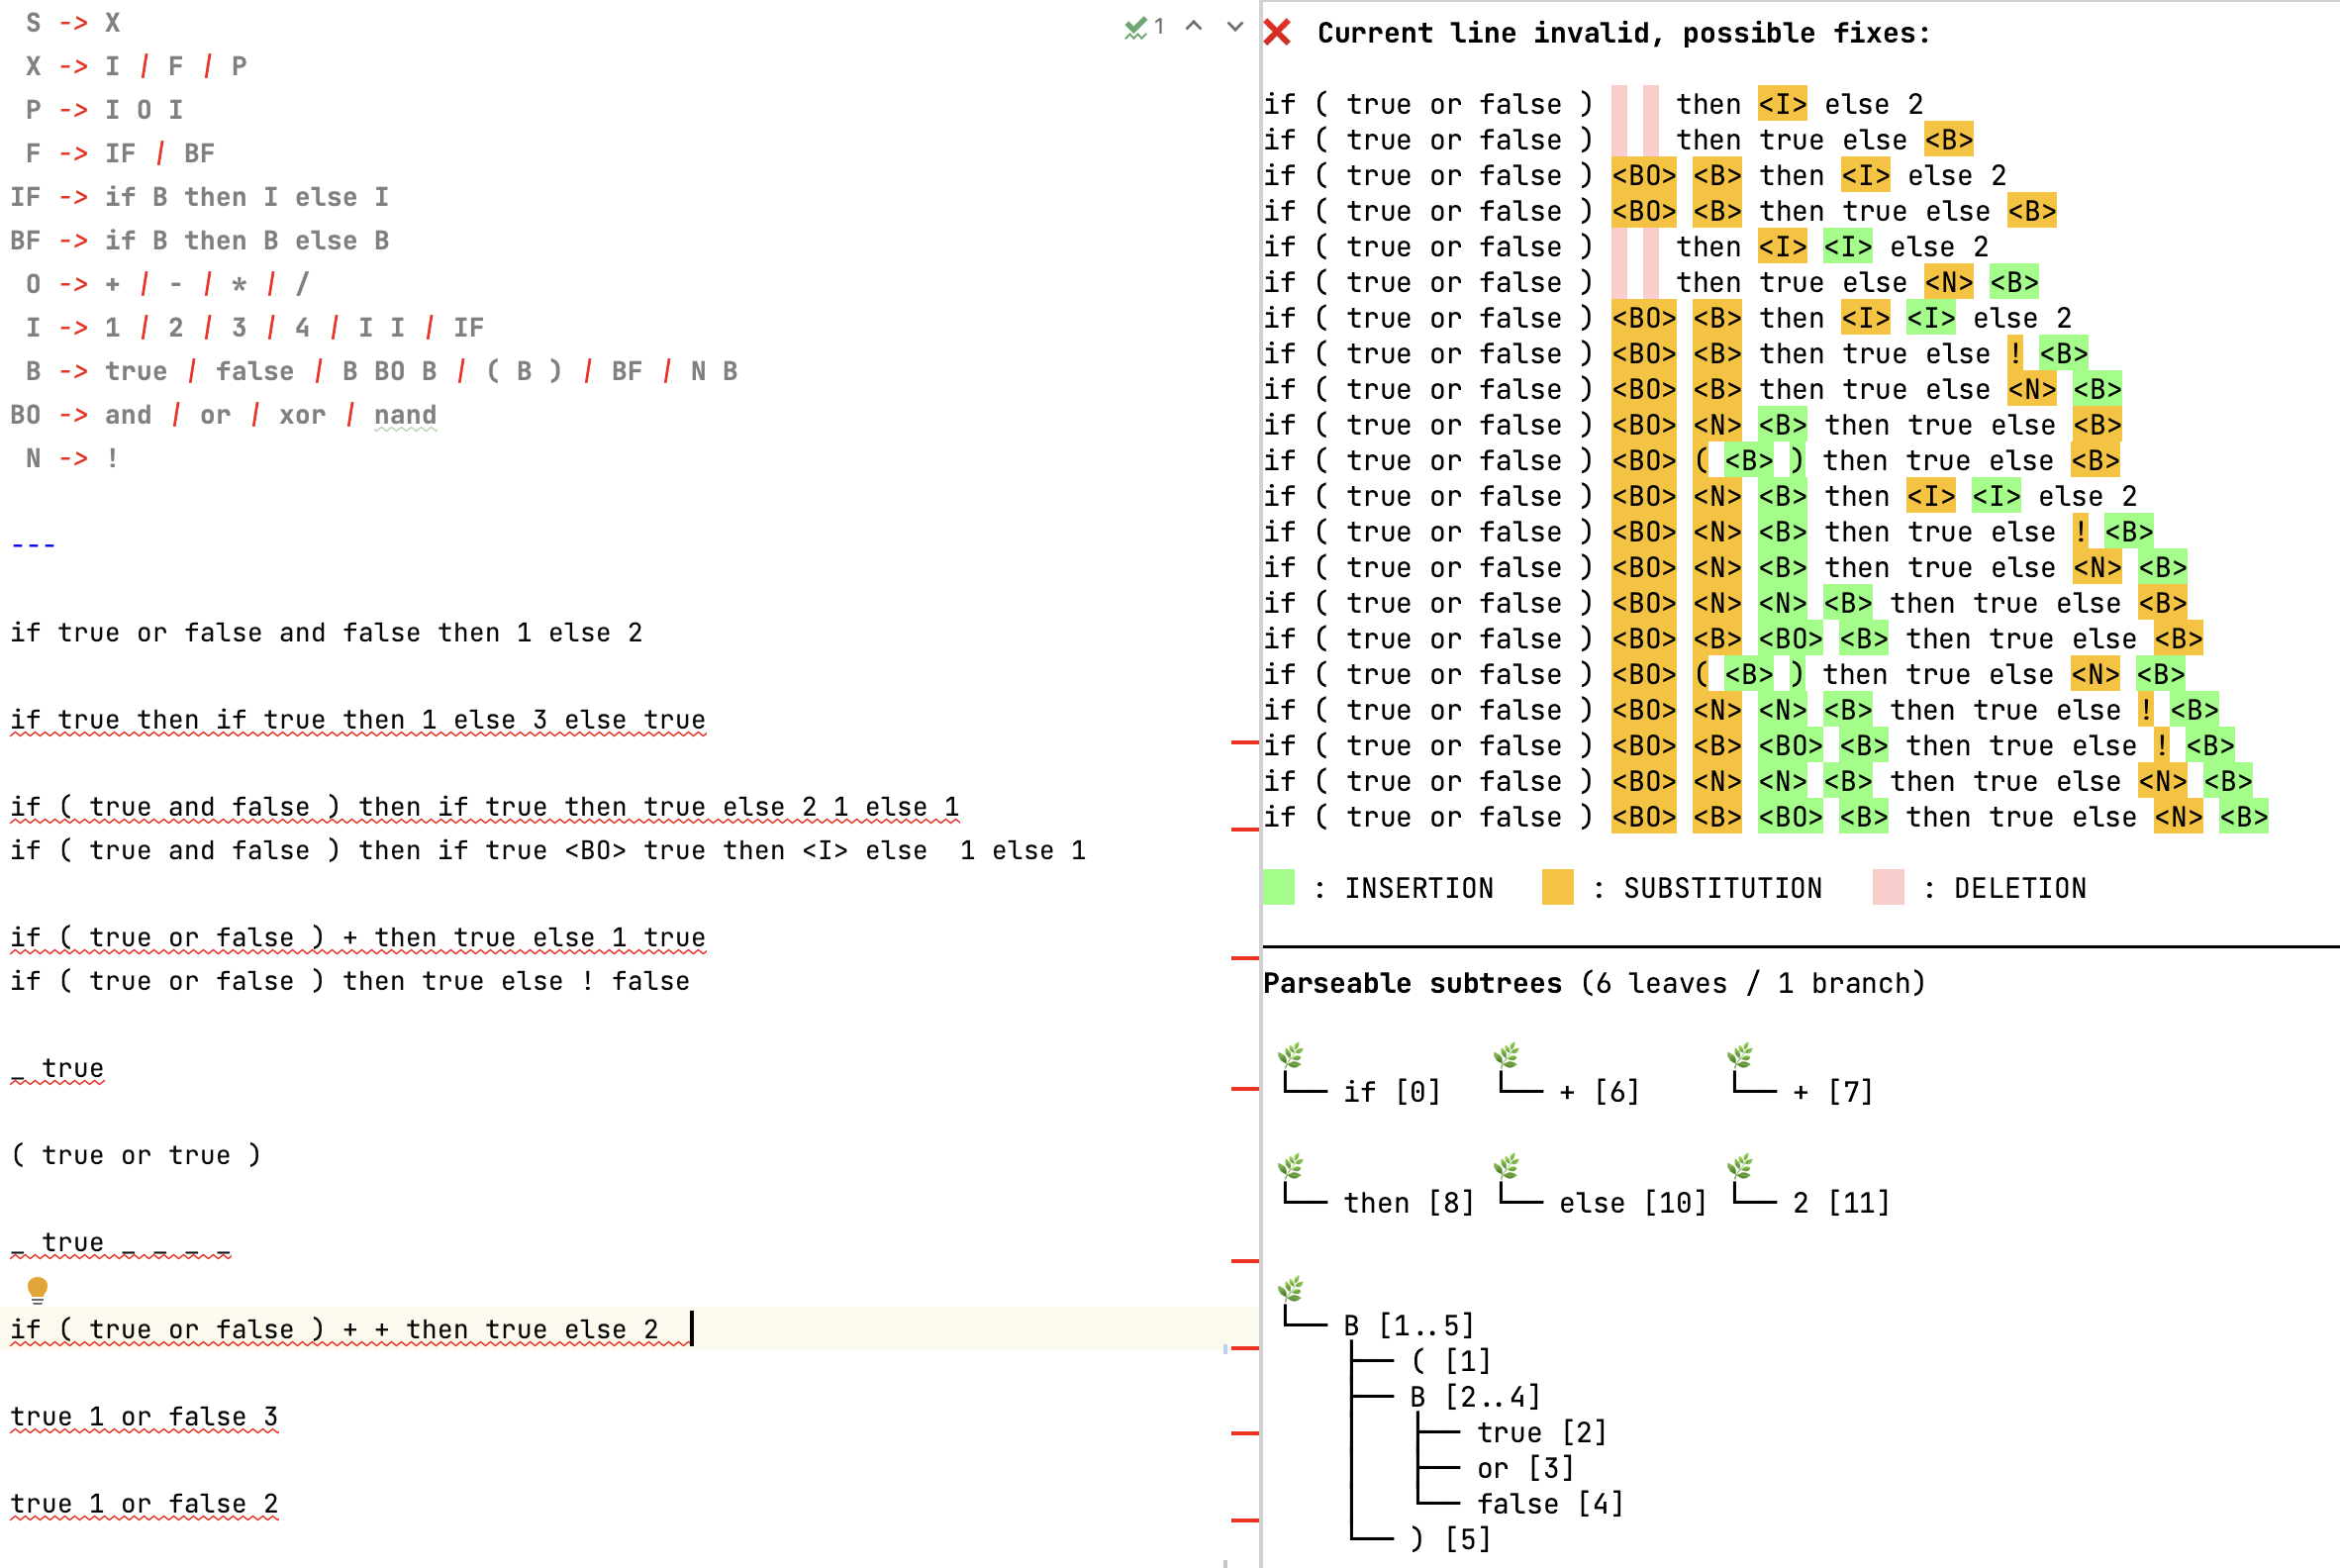
\includegraphics[width=\textwidth]{tidyparse_screenshot.png}}
        \end{minipage}

        \jointspacing

        \mysection{Idiolect}

        \null\hspace*{1.8cm}\begin{minipage}[c]{0.90\columnwidth}
                                Bind custom phrases in a reconfigurable IDE plugin with instant adaptation.\\

                                \href{https://github.com/openasr/idiolect}{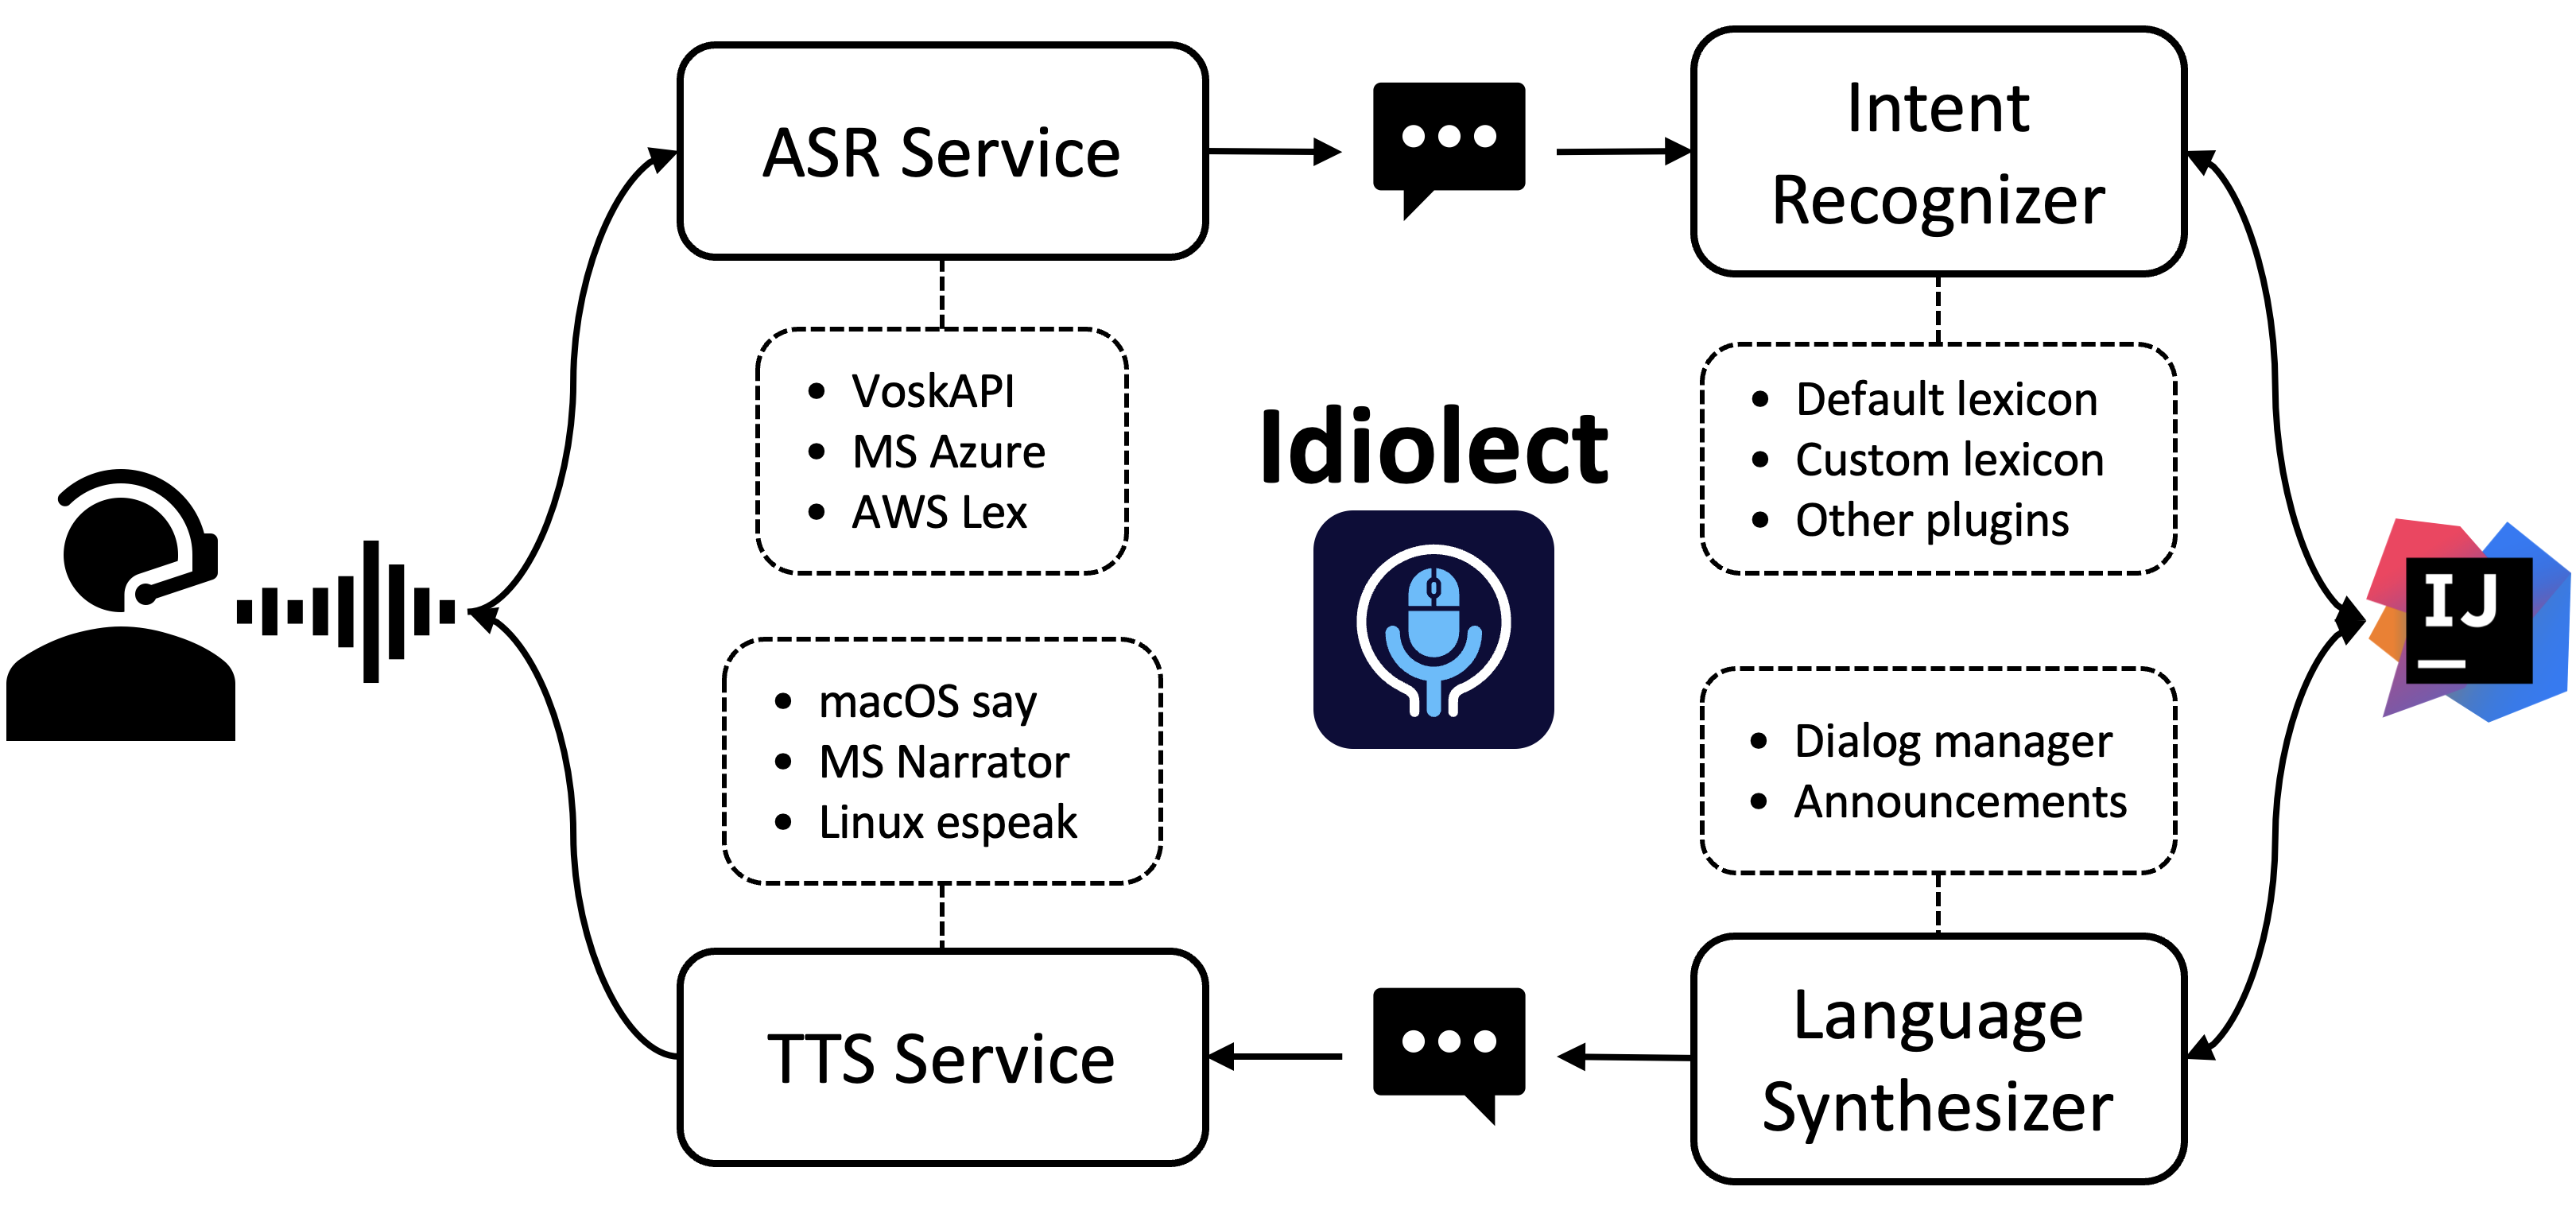
\includegraphics[width=\textwidth]{architecture.png}}
        \end{minipage}

        \jointspacing

    \end{multicols}

    \bottombox{
    %% QR code
    %    \hfill\bottomboxlogo{img/kotlin_logo.png}
    % Comment out the line below out to hide logo
        \begin{minipage}[c][0.1\paperheight][c]{0.18\textwidth}\qrcode[height=2.6in]{teach.ndan.co} \end{minipage}
        \hspace{-2.5cm}\begin{minipage}[l][0.1\paperheight][c]{0.33\textwidth}
\includegraphics[height=2.6in]{mcgill.png} \end{minipage}
        \hspace{-4.5cm}\begin{minipage}[l][0.1\paperheight][c]{0.33\textwidth}
\includegraphics[height=2.6in]{mila.png} \end{minipage}
        \hspace{-10cm}\begin{minipage}[c][0.1\paperheight][c]{0.20\textwidth}
\includegraphics[height=2.6in]{icons.png} \end{minipage}

    %    \hfill\bottomboxlogo{img/mila_mauve.png} % \hfill shifts the logo across so it meets the right hand side margin
    % Note that \bottomboxlogo takes an optional width argument. It defaults to the following:
    % \hfill\bottomboxlogo[width=\textwidth]{<path_to_image_file>}
    % where \textwidth is actually the width of a minipage which is defined in the \bottombox command of
    % betterportaitposter.cls It's a standard \includegraphics command in there, so easy to change if
    % you need to add a border etc.
    }
\end{poster}
\end{document}
